%% Version 4.3.2, 25 August 2014
%
%%%%%%%%%%%%%%%%%%%%%%%%%%%%%%%%%%%%%%%%%%%%%%%%%%%%%%%%%%%%%%%%%%%%%%
% Template.tex --  LaTeX-based template for submissions to the 
% American Meteorological Society
%
% Template developed by Amy Hendrickson, 2013, TeXnology Inc., 
% amyh@texnology.com, http://www.texnology.com
% following earlier work by Brian Papa, American Meteorological Society
%
% Email questions to latex@ametsoc.org.
%
%%%%%%%%%%%%%%%%%%%%%%%%%%%%%%%%%%%%%%%%%%%%%%%%%%%%%%%%%%%%%%%%%%%%%
% PREAMBLE
%%%%%%%%%%%%%%%%%%%%%%%%%%%%%%%%%%%%%%%%%%%%%%%%%%%%%%%%%%%%%%%%%%%%%

%% Start with one of the following:
% DOUBLE-SPACED VERSION FOR SUBMISSION TO THE AMS
\documentclass{ametsoc}

% TWO-COLUMN JOURNAL PAGE LAYOUT---FOR AUTHOR USE ONLY
% \documentclass[twocol]{ametsoc}

%%%%%%%%%%%%%%%%%%%%%%%%%%%%%%%%
%%% To be entered only if twocol option is used

\journal{jtech}

%  Please choose a journal abbreviation to use above from the following list:
% 
%   jamc     (Journal of Applied Meteorology and Climatology)
%  jtech     (Journal of Atmospheric and Oceanic Technology)
%   jhm      (Journal of Hydrometeorology)
%   jpo     (Journal of Physical Oceanography)
%   jas      (Journal of Atmospheric Sciences)	
%   jcli      (Journal of Climate)
%   mwr      (Monthly Weather Review)
%   wcas      (Weather, Climate, and Society)
%   waf       (Weather and Forecasting)
%   bams (Bulletin of the American Meteorological Society)
%   ei    (Earth Interactions)

%%%%%%%%%%%%%%%%%%%%%%%%%%%%%%%%
%Citations should be of the form ``author year''  not ``author, year''
\bibpunct{(}{)}{;}{a}{}{,}

%%%%%%%%%%%%%%%%%%%%%%%%%%%%%%%%

%%% To be entered by author:

%% May use \\ to break lines in title:

\title{Estimating $\chi$ and $K_T$ from fast-reponse thermistors on traditional shipboard CTDs: sources of uncertainty and bias.}

%%% Enter authors' names, as you see in this example:
%%% Use \correspondingauthor{} and \thanks{Current Affiliation:...}
%%% immediately following the appropriate author.
%%%
%%% Note that the \correspondingauthor{} command is NECESSARY.
%%% The \thanks{} commands are OPTIONAL.

    %\authors{Author One\correspondingauthor{Author One, 
    % American Meteorological Society, 
    % 45 Beacon St., Boston, MA 02108.}
% and Author Two\thanks{Current affiliation: American Meteorological Society, 
    % 45 Beacon St., Boston, MA 02108.}}

\authors{Andy Pickering\correspondingauthor{College of Earth, Ocean, and Atmospheric Sciences, Oregon State University,Corvallis, OR.}}

%% Follow this form:
     \affiliation{College of Earth, Ocean, and Atmospheric Sciences, Oregon State University,Corvallis, OR.}

%\affiliation{}

%% Follow this form:
    %\email{latex@ametsoc.org}

\email{}

%% If appropriate, add additional authors, different affiliations:
    \extraauthor{Jonathan Nash}
    \extraaffil{College of Earth, Ocean, and Atmospheric Sciences, Oregon State University,Corvallis, OR.}

    \extraauthor{Jim Moum}
    \extraaffil{College of Earth, Ocean, and Atmospheric Sciences, Oregon State University,Corvallis, OR.}

    \extraauthor{Jen MacKinnon}
    \extraaffil{UCSD / Scripps Institute of Oceanography}



%\extraauthor{}
%\extraaffil{}

%% May repeat for a additional authors/affiliations:

%\extraauthor{}
%\extraaffil{}

%%%%%%%%%%%%%%%%%%%%%%%%%%%%%%%%%%%%%%%%%%%%%%%%%%%%%%%%%%%%%%%%%%%%%
% ABSTRACT
%
% Enter your abstract here
% Abstracts should not exceed 250 words in length!
%
% For BAMS authors only: If your article requires a Capsule Summary, please place the capsule text at the end of your abstract
% and identify it as the capsule. Example: This is the end of the abstract. (Capsule Summary) This is the capsule summary. 

\abstract{The acquisition of turbulence data from traditional shipboard CTD casts is attractive, as it has the potential to dramatically increase the amount of deep-ocean mixing observations globally.  While data from shear-probes are easily contaminated by motion of the instrument platform, the measurement of temperature gradient is relatively insensitive to vehicle vibration, making it possible to measure temperature gradient from a shipboard CTD rosette.  The purpose of this note is to investigate the error and bias in estimating the rate of dissipation of temperature variance $\chi$ and turbulent diffusivity $K_T$ from traditional CTD casts.  The most significant source of error is associated with the fact that fast-response FP07 thermistors resolve only a fraction of the temperature gradient variance at the fallspeed of typical CTD casts.  Assumptions must be made about the wavenumber extent of the temperature gradient spectrum, which scales with the rate of dissipation of tubulent kinetic energy, a quantity that is not directly measured.  Here we utilize observations from a microstructure profiler to demonstrate the validity of the method of estimating $\chi$ from thermistor data, and to assess uncertainty and bias. We then apply this methodology to temperature gradient profiles obtained from $\chi$pods mounted on a CTD (the CTD-$\chi$-pod), and compare these to microstructure profiles obtained almost synoptically at the equator.  CTD-$\chi$-pod estimates of $\chi$ compare favorably to the direct microstructure measurements and demonstrate that the $\chi$-pod method is not significantly biased.  This supports the utility of the measurement as part of the global repeat hydrography program (GO-SHIP) cruises, during which this type of data has been acquired during the past few years.}


\begin{document}

%% Necessary!
\maketitle


%%%%%%%%%%%%%%%%%%%%%%%%%%%%%%%%%%%%%%%%%%%%%%%%%%%%%%%%%%%%%%%%%%%%%
% MAIN BODY OF PAPER
%%%%%%%%%%%%%%%%%%%%%%%%%%%%%%%%%%%%%%%%%%%%%%%%%%%%%%%%%%%%%%%%%%%%%
%

%% In all cases, if there is only one entry of this type within
%% the higher level heading, use the star form: 
%%

% \section{Introduction}
% \subsection*{subsection}
% text...
% \section{Section title}

%vs

% \section{Section title}
% \subsection{subsection one}
% text...
% \subsection{subsection two}
% \section{Section title}

%%%
% \section{First primary heading}

% \subsection{First secondary heading}

% \subsubsection{First tertiary heading}

% \paragraph{First quaternary heading}


%~~~~~~~~~~~~~~~~~~~~~~
\section{Introduction}
%~~~~~~~~~~~~~~~~~~~~~~

Turbulent mixing affects the distribution of heat, salt, and nutrients throughout the global ocean. Diapycnal mixing  of cold, dense water with warmer water above maintains the abyssal overturning circulation \citep{munk66,munkwunsch98}, which affects global climate. Because the turbulence that drives mixing generally occurs at scales that are not resolved in climate models, it must be parameterized, based on either (i) aspects of the resolved model dynamics, (ii) through higher resolution models that capture the dynamics that feed energy to turbulence, or (iii) using other parameterizations that either dynamically or statistically quantify turbulent fluxes. Recent investigations have demonstrated that these models are sensitive to the magnitude and distribution of mixing \citep{meletetal13}. A comprehensive set of measurements that spans relevant dynamical regimes is needed to constrain mixing and develop more accurate parameterizations.

Direct measurement of mixing with microstructure profilers equipped with shear probes is expensive, time-intensive, and requires considerable care and expertise. Moreover, tethered profilers can't reach abyssal depths, requiring autonomous instruments to get deeper than $\sim$1000-2000 m.  As a result, existing measurements of diapycnal mixing, especially in the deep ocean, are sparse \citep{waterhouseetal14}. In order to obtain a larger quantity of mixing estimates, considerable work has gone into inferring mixing from measurements of the outer scales of turbulence, which are easier to obtain. One popular method is the use of Thorpe scales, where diapycnal mixing is inferred from inversions in profiles of temperature or density  \citep{thorpe77,dillon82}. The size of resolvable overturn is limited by the profiling speed and instrument noise \citep{galbraithkelley96}. Several studies indicate relatively good agreement with microstructure and other observations, but there are some questions about the validity of the method and the assumptions made \citep{materetal15,scotti15}. Parameterizations based on profiles of shear and/or strain have also been developed and applied to estimate diapycnal mixing \citep{gregg89a,kunzeetal06,polzinetal13,whalenetal12,whalenetal15}.  However, they rely on a series of assumptions about the cascade of energy from large to small scales that are often violated; numerous studies (i.e., \cite{watermanetal13}) have shown that there is significant uncertainty associated with these parameterizations, in that there can be a consistent bias in a particular region, yet the sense of the bias (i.e., overpredict vs.\ underpredict) is not known a priori. 

Quanitifying turbulence from velocity shear variance (to compute the dissipation rate of turbulent kinetic energy $\epsilon$) is challenging on moorings or profiling platforms because there is usually too much vibration and/or package motion for shear-probes to be useful. Other methods (i.e., optics or acoustics) may hold some promise, but lack of scatterers often precludes this type of measurement, especially in the abyss.  In addition, shear probes only provide $\epsilon$, not the mixing of scalars, $K$, which is often inferred from $\epsilon$ by assuming a mixing efficiency $\Gamma$ \citep{osborn80} as $K=\Gamma \epsilon / N^{2}$, which $N^2$ is the buoyancy frequency.  A more direct measure of turbulent mixing is obtained from the dissipation rate of temperature variance $\chi$ \citep{osborncox72}.  This has the advantage that (i) the temperature and temperature gradient can be computed and is relatively straightforawrd to measure, and (ii) the estimation of mixing from $\chi$ does not require assumptions about $\Gamma$. However, the spectrum of temperature gradient extends to very small scales, so that its spectrum is seldom fully resolved (and unlike shear variance, the wavenumber extent of the temperature gradient spectrum does not scale with its amplitude, but instead depends on $\epsilon$). Assumptions about the spectral shape (Kraichnan vs.\ Bachelor, and the value of the ``constant'' q) and its wavenumber extent (governed by the Batchelor wavenumber $k_b=[\epsilon/(\nu D_{T}^{2})]^{1/4}$  \citep{Batchelor59}) are thus necessary to determine $\chi$ unless measurements capture the full viscous-diffusive subrange of turbulence (i.e., down to scales $\Delta x \sim 1/k_b \sim 1$mm), a criterion seldom achieved.  To resolve this, we follow \cite{alfordpinkel00b} and \cite{moumnash09} and make the assumption that $K_T=K_{\rho}$ to determine the dissipation rate as $\epsilon_{\chi}=(N^2\chi)/(2\Gamma <dT/dz>^2)$, permitting $k_b$ to be estimated. 


The goal of this paper is to outline and validate the methods used to compute $\chi$ and $K_T$ with $\chi$-pods mounted on CTDs.  We do this by applying our processing methodology to profiles of temperature gradient measured by thermistors on the `Chameleon' microstructure profiler, which provides a direct test of our methodology.  Because Chameleon is a loosely tethered profiler equipped with shear probes (Moum et al 1995), it directly measures $\epsilon$ and allows us to test our assumptions.  Specifically, it allows us to determine biases associated with computing $\chi$ from partially-resolved temperature alone, as compared to that when it is computed by including knowledge of the dissipation rate, which constrains the wavenumber extent of the scalar spectra.   After establishing that the method works, we then compare CTD-$\chi$pod profiles to nearby microstructure profiles.


%~~~~~~~~~~~~~~~~~~~~~~
\section{Data }
%~~~~~~~~~~~~~~~~~~~~~~


%~~~~~~~~
\subsection{EQ14}

Data were collected on the R/V Oceanus in Fall 2014 during the EQ14 experiment to study equatorial mixing.  More than 2700 Chameleon profiles were made, along with 35 CTD-$\chi$pod profiles bracketed by Chameleon profiles in order to maintain calibrations during the cruise. Most Chameleon profiles were made to a maximum depth of about 250m, with CTD casts going to 500m or deeper. The EQ14 experiment and results are discussed in more detail in ( SJ Warner, RN Holmes, EH McHugh-Hawkins, JN Moum, 2016: Buoyant gravity currents released from tropical instability waves, JPO, in preparation).




%~~~~~~~~~~~~~~~~~~~~~~
\section{Methods}
%~~~~~~~~~~~~~~~~~~~~~~
%~~~~~~~~

%Also, you might want to include a figure showing something about removing depth loops (like the figure in the proposal), and then also quantify how much data needs to be thrown out as a function of sea-state.  All of this was in the proposal.    

As mentioned in the introduction, the temperature gradient spectrum is rarely fully resolved down to the small scales of turbulent mixing. The fraction of the spectrum resolved depends on the true spectrum (a function of $\chi$ and $\epsilon$), the flowspeed past the sensor ($u$), and the response of the thermistor. The GE/Thermometrics FP07 thermistors we use typically resolve frequencies up to about 10-15 Hz. The maximum resolved wavenumber is then equal to $k_{max}=f_{max}/u$, while the wavenumber extent of the true spectrum varies with $k_b$ (and $\epsilon^{1/4}$). At the typical vertical fall rate of a CTD rosette ($\sim$1m/s), only about 20\% of $k_b$ is resolved at $\epsilon=10^{-10}Wkg^{-1}$ (Figure \ref{kbratVseps}). While methods have been developed to fit the observed temperature gradient spectrum to theoretical forms \citep{ruddicketal00}, these work only when a larger fraction of the temperature gradient spectrum is resolved. For the relatively high profiling speeds typical of CTD casts, we find these methods do not work well (see appendix for details) and therefore we use the following methodology, which does not have a strongly $\epsilon$-dependent bias.

We first outline our method for estimating $\chi$, which relies on (i) determining the instantaneous flowspeed past the sensor, (ii) identfying periods where the signals may be contaminated by the wake of the CTD rosette, (iii) defining the relavent $N^2$ and $(dT/dz)^2$, and (iv) applying an iterative method to compute $\chi$ and $K_T$. We then discuss some limitations and practical considerations that arise.

\subsection{Iterative Method for estimating $\chi$}

For each $\sim$1 second window, $\chi$ is estimated via the following procedure as outlined in \cite{moumnash09}. For isotropic turbulence,
\begin{equation}
\chi_T=6D_T \int_{0}^{\infty}\Psi_{T_x} (k) dk
\label{eq:chiint}
\end{equation}
where $D_T$ is the thermal diffusivity and $\Psi_{T_x} (k)$ is the wavenumber spectrum of $dT/dx$.

Note that $dT/dx$ is not actually measured; $dT/dt$ is measured, and $dT/dx$ is inferred from Taylor's frozen flow hypothesis:
 \begin{equation}
\frac{dT}{dx}=\frac{1}{u}\frac{dT}{dt}
\label{eq:2}
\end{equation}

The wavenumber extent of the spectrum depends on the Batchelor wavenumber $k_b$, which is related to $\epsilon$:
\begin{equation}
k_b=[\epsilon/(\nu D_{T}^{2})]^{1/4}
\label{eq:3}
\end{equation}

We assume that $K_{\rho}=K_T$ and $K_{\rho}=\Gamma \epsilon /N^2$. Then dissipation rate is computed as
\begin{equation}
\label{eq:eps}
\epsilon_{\chi}=\frac{N^2\chi_T}{2\Gamma <dT/dz>^2}
\end{equation}

Typical thermistors do not resolve the spectrum out to $k_b$, so the measured spectrum is fit to the Kraichnan form of theoretical scalar spectrum over the range of resolved wavenumbers ($k_{min}<k<k_{max}$).The variance between the measured $[\Phi_{T_x}(k)]_{obs}$ and theoretical $[\Phi_{T_x}(k)]_{theory}$ spectra at these wavenumbers is assumed to be equal:

\begin{equation}
\int^{k_{max}}_{k_{min}}[\Phi_{T_x}(k)]_{obs}dk=\int^{k_{max}}_{k_{min}}[\Phi_{T_x}(k)]_{theory}dk
\label{eq:speceq}
\end{equation}

An iterative procedure is then used to fit and calculate $\chi$ and $\epsilon$:

\begin{enumerate}
\item First we estimate $\chi_T$ based on an initial guess of $\epsilon=10^{-7}$ $\mathrm{Wkg^{-1}}$ and compute $k_b$ via eq. \ref{eq:3}. We set $k_{max} = k_b/2$ or to a wavenumber equivalent to $f_{max}=7$ Hz [i.e., $k_{max}= 2\pi(f_{max})/u$], whichever is smaller. We choose $f_{max}=7$Hz because the thermistors' response rolls off at higher frequencies (see appendix for more details).
\item We then use Eq. (\ref{eq:eps}) to refine our estimate of $k_b$ and recompute $\chi_T$ using Eqs. (\ref{eq:chiint}) and (\ref{eq:speceq}). 
\item This sequence is repeated and converges after two or three iterations.
\end{enumerate}
Note that this procedure is equivalent to the explicit formulation of \citep{alfordpinkel00b}, except we use the Kraichnan theoretical form instead of the Batchelor spectrum for $[\Phi_{T_x}(k)]_{theory}$.

\subsection{CTD-$\chi$pod Data Processing}

The basic outline for processing each CTD-$\chi$-pod profile is as follows:
\begin{enumerate}
\item The correct time-offset for the $\chi$-pod clock is determined by aligning $dp/dt$ from the 24Hz CTD data to vertical velocity calculated by integrating vertical accelerations measured by the $\chi$-pod. $\chi$-pod clock drift is small, typically on the order of 1 sec/week, but it is imperative to get records aligned within $< 0.5$ s so that the correct $u = w = d p/dt$ is used.
\item Low-order polynomial calibration coefficients are determined to convert thermistor voltages from $\chi$pod to ITS90 temperature (as measured by
the CTD). Figure \ref{f2} shows an example of the aligned and calibrated CTD-$\chi$pod timeseries for one cast. Note the significant differences in amount of variance associated with the two sensors during down and up casts. For the upward-mounted sensor (T1), the downcast signal is associated with the CTD wake, as is the upcast for the downward-mounted sensor (T2). Only the `clean' portions of the cast (e.g., the T1 upcast and the T2 downcast) are used in the $\chi$pod calculations.
\item Depth loops are identified and flagged in the 24Hz CTD data. $\chi$-pod data during these times are discarded since the signals are likely contaminated by the wake of the CTD. Even for profiles that are significantly affected by ship heaving, good segments of data are obtained over a majority of the depths after removing contaminated data. * include figure and include criteria for identifying loops *
\item Buoyancy frequency $N^2$ and temperature gradient $dT/dz$ are computed from 1-m binned CTD data, and averaged over a scale of 10m. The results are not very sensitive to the averaging interval (see appendix for more details).
\item Half-overlapping 1 sec windows of data are used to estimate $\chi$, $\epsilon$, and $K_T$ following the methods described in \cite{moumnash09}, as outlined in the previous section.
\end{enumerate}


%%~~~~~~
\subsection{Example Spectra and Fits}

Examples of the observed and fit spectra are shown in Figure \ref{specexamp}, for low and high dissipation rate. Note that at lower $\epsilon$, a larger fraction of $k_b$ is observed and the peak of the spectrum is nearly resolved. At higher $\epsilon$, less of the spectrum is resolved and the spectral peak is well above the maximum resolved wavenumber. Even so, the iterative $\chi$pod method gives an accurate estimate of $\chi$. Also note that errors in $\epsilon$ can be larger, even when $\chi$ is accurate; the shape of the spectrum at resolved wavenumbers is not sensitive to $\epsilon$?. 



%~~~~~~~~~~
\subsection{flowspeed past the sensor}

The flowspeed past the thermistor is needed to convert the measured temperature derivative $dT/dt$ to a spatial gradient. For the CTD-$\chi$pod, the largest contribution to the flowspeed is usually the vertical velocity of the CTD package ($dp/dt$), which is close to 1m/s on average, so we typically neglect the horizontal component of velocity in converting from frequency to wavenumber spectra. Although this will be a good approximation, errors may be introduced where horizontal velocities are large. Note that because it is the total instantaneous velocity magnitude that represents flow past the sensor, neglecting the horizonal component of velocity (assuming $u=dp/dt$) means we are always underestimating the true flowspeed past the sensor. When the CTD package is equipped with LADCP, the true flowspeed can be measured. In some cases (including EQ14) where the CTD was not equipped with LADCP, it would seem that the ship's ADCP could be used to estimate the horizontal component of velocity. However, because the CTD does not travel perfectly vertically in strong currents, this is difficult to do in practice. In a strong horizontal flow, the CTD will drift with the current while descending, lowering the flow relative to the sensors. On the upcasts, the CTD will be pulled against the current, increasing the flow relative to the sensors. Since the CTD in EQ14 was not equipped with LADCP, we use $dp/dt$ as the flowspeed, and estimate potential errors in the appendix.

%%~~~~~~~~~~~~~~~~~~~~~~
%\section{Oceanographic Setting and Conditions}
%%~~~~~~~~~~~~~~~~~~~~~~
%
%Brief overview of dynamics in study region? More details are given in Warner et al (in prep).


%~~~~~~~~~~~~~~~~~~~~~~
\section{Results }
%~~~~~~~~~~~~~~~~~~~~~~


\subsection{Direct Test of $\chi$pod Method}

We begin by utilizing the highly-resolved turbulence profiler data (for which both $\epsilon$ and $\chi$ are measured) to test the assumptions in our method of estimating $\chi$. We first apply the $\chi$pod method to each Chameleon profile, using only the FP07 thermistor data. These results, which we will refer to as $\chi_{\chi}$, are then compared with $\chi_{\epsilon}$, computed by integrating the theoretical temperature gradient spectrum with $k_b$ computed directly from shear-probe derived $\epsilon$. Qualitatively, $\chi_{\chi}$ and $\chi_{\epsilon}$ show very similar depth and time patterns (Figure \ref{eq14_eps_pcolor}) and appear to agree in magnitude, suggesting the method works well. A more quantitative comparison is made with a 2-D histogram (Figure \ref{eq14_chi_2dhist}), showing the two are well-correlated over a wide range of magnitudes. The distribution of $log_{10}$ of the $\chi$ ratios is approximately normal, with a mean of $\mu=0.15$ and standard deviation of $\sigma=0.54$. 



%~~~~~~~~~~~~~~~~~~~~~~
\subsection{ CTD$\chi$-pod - Chameleon Comparison}
%~~~~~~~~~~~~~~~~~~~~~~

Having demonstrated that the method works for Chameleon data, we now compare $\chi$ from CTD-mounted $\chi$pods to $\chi_{\epsilon}$. In contrast to the Chameleon data, the CTD is more strongly coupled to the ship, and therefore subject to more vibration, heaving, and artifical turbulence created by the rosette. A total of 35 CTD-$\chi$pod casts were performed, bracketed with Chameleon profiles immediately before and after. We first compare CTD-$\chi$pod profiles to the mean of the two Chameleon profiles bracketing each cast, both averaged in 5m depth bins (Figure \ref{eq14_cdtChi_vs_cham}). The two are correlated, with considerable scatter but no apparent bias. Since we expect significant natural variability even between adjacent Chameleon profiles, we investigate further to determine if the observed $\chi$pod variability is of a similar magnitude or greater than expected. Scatter plots of before vs. after Chameleon profiles (not shown), typically separated by about an hour, show a similar level of scatter as the differences between methods, suggesting that the observed differences (Figure \ref{eq14_cdtChi_vs_cham}) can be explained by natural variability in turbulence. This is demonstrated by histograms of the ratio of $\chi$ from adjacent casts (Figure \ref{eq14_cdtChi_vs_cham_hist}) which show that the variability between CTD $\chi$pod and Chameleon casts is similar to the natural variability between before/after Chameleon profiles. Profiles from all CTD-Chameleon pairs averaged in time and 40m depth bins (Figure \ref{ctd_cham_chi_boot_all}) overlap within 95\% confidence limits at all depths where there exists good data for both. Averages of subsets of these profiles that were clustered in position/time (not shown) also agree well. We conclude that the variability between CTD$\chi$pod and Chameleon profiles is indistinguishable from natural variability in turbulence levels.


%~~~~~~~~~~~~~~~~~~~~~~
\section{Discussion}
%~~~~~~~~~~~~~~~~~~~~~~

We have shown that $\chi$ can be accurately estimated from $\chi$pods attached to CTD rosettes. The method also estimates $\epsilon$, but we have not discussed it here since it involves more assumptions and uncertainties. One major assumption is the mixing efficiency $\Gamma$. A value of $0.2$ is commonly assumed, but evidence suggests this may vary significantly (see appendix for a study of the sensitivity to this parameter). Another major assumption in the $\chi$pod method is that $K_T=K_{\rho}$. Preliminary investigation on this data suggests that this assumption does not hold here and may be responsible for a negative bias in $\epsilon$, but more work is needed to verify this. However we have shown that even if $\epsilon$ estimates are biased, $\chi$ and $K_T$ are still robust.

The goal of CTD-$\chi$pods is to expand the number and spatial coverage of ocean mixing observations. We have already deployed instruments during several process experiments and on several GO-SHIP repeat-hydrography cruises. We plan to continue regular deployment on GO-SHIP and similar cruises, adding $\chi$ and $K_T$ to the suite of variables regularly measured. The expanding database of mixing measurements from CTD-$\chi$pods will also enable testing of other commonly-used or new mixing parameterizations. This has the potential to be transformative, allowing the community to 
develop and test global turbulence parameterizations, use estimates of turbulence along with the CLIVAR repeat hydrography data for inverse models and water mass modification calculations, identify hotspots of turbulence to target with future process experiments, and compare with in-situ chemical and biological measurements made routinely on repeat hydrography cruises.

% thanks Jen for some of above text!

%~~~~~~~~~~~~~~~~~~~~~~
\section{Conclusions}
%~~~~~~~~~~~~~~~~~~~~~~

\begin{itemize}
\item The $\chi$pod method for estimating $\chi$ and $K_T$ was directly applied to temperature gradients measured by the Chameleon microstructure profiler on $>$ 2700 profiles during the EQ14 cruise. The estimated $\chi_{\chi}$ agrees well with $\chi_{\epsilon}$ calculated using $\epsilon$ from shear probes over a wide range of magnitudes (Figure \ref{eq14_chi_2dhist}) with little or no bias, demonstrating that the method works.
\item CTD-$\chi$pod profiles were also compared to nearby Chameleon profiles during the cruise. Variability between CTD-$\chi$pod and Chameleon estimates of $\chi$ is indistinguishable from natural variability between Chameleon profiles. Time-averaged profiles of $\chi$ from both platforms agree within 95\% confidence limits, and no significant bias was detected between the estimates of $\chi$.
\item We conclude that estimates of $\chi$ and $K_T$ made from the CTD-$\chi$pod platform are robust and reliable.
\end{itemize}



%%%%%%%%%%%%%%%%%%%%%%%%%%%%%%%%%%%%%%%%%%%%%%%%%%%%%%%%%%%%%%%%%%%%%
% ACKNOWLEDGMENTS
%%%%%%%%%%%%%%%%%%%%%%%%%%%%%%%%%%%%%%%%%%%%%%%%%%%%%%%%%%%%%%%%%%%%%
%
\acknowledgments
%Harper Simmons provided microstructure data. Data were collected during IWISE, which was funded by ONR. Others...
The EQ14 experiment was funded by ???. We thank the Captain and crew of R/V Oceanus. Also thank people who helped collect the data, those who made the sensors, etc..


%%%%%%%%%%%%%%%%%%%%%%%%%%%%%%%%%%%%%%%%%%%%%%%%%%%%%%%%%%%%%%%%%%%%%
% APPENDIXES
%%%%%%%%%%%%%%%%%%%%%%%%%%%%%%%%%%%%%%%%%%%%%%%%%%%%%%%%%%%%%%%%%%%%%
%
% Use \appendix if there is only one appendix.
%\appendix

% Use \appendix[A], \appendix}[B], if you have multiple appendixes.
%\appendix[A]

%% Appendix title is necessary! For appendix title:
%\appendixtitle{Sensitivity to `fmax'}
%
%Here we investigate the sensitivity of the $\chi$pod calculations to the parameter `fmax', the upper limit for integrating the temperature gradient spectrum. In practice, fmax is limited by the frequency at which the FP07 thermistor rolls off. This varies slightly between individual thermistors, but is typically between 10-15 Hz for the sensors we use (show example spectra?). Figure ? shows $\chi_{\chi}$ vs $\chi_{\epsilon}$ for different values of fmax. 


\appendix[A]

%% Appendix title is necessary! For appendix title:
\appendixtitle{Sensitivity Analysis}

\section{Flowspeed Past Sensor}

We investigated the potential error in the $\chi$pod calculations from ignoring horizontal velocities and assumed the flow speed is equal to the vertical speed of the CTD rosette, determined from the recorded pressure $dp/dt$. To quanitify this error, we repeated the calculations with constant offsets added to the flowspeed. Since the total magnitude of velocity is used, $dp/dt$ is a minimum estimate of the true speed. Adding $0.1$($1$)m/s results in a mean percent error of 6(40) percent (Figure \ref{FspdSensHist}), small compared the large natural variability in turbulence and uncertainty in our measurements. Note that increasing the velocity tends to result in smaller values of $\chi$, since it shifts the spectrum to lower wavenumbers. 

We also looked for any systematic biases associated with flowpseed. We found the $\chi$ was biased high for very small speeds ($u<25$cm/s). This could be assoicated with contamination by CTD wake or entrained water when the CTD slows.  These values were discarded for our analysis.

%\appendix[B]

%\clearpage
%~~~~~~~~~~~~~~~~~~~~~~~~~
%\appendixtitle{Sensitivty to $\Gamma$, $N^2$ and $dT/dz$ }

\section{$N^2$ and $dT/dz$}

We investigated the sensitivity of the calculations to the scale over which $N^2$, $dT/dz$ are averaged. The iterative method to estimate chi requires the background stratification $N^2$ and temperature gradient $dT/dz$. The estimate of $\chi$ is insenstive to these scales. However, while dissipation rate $\epsilon$ and diffusivity $K_T$ are more strongly affected because they are linearly related to these values. Computing $N^2$ and $dT/dz$ over smaller scales results in larger values and hence some larger values of $K_T$.

\section{Mixing Efficiency}

We also examined the sensitivity to the value of the mixing efficiency $\Gamma$. A value of $0.2$ is commonly assumed, although several studies have indicated it could be different or variable. We used several values and compared each to the reference case of $\Gamma=0.2$. Values of $\chi$ ranged up to $\pm$2 times the reference values.


\appendix[B]

%% Appendix title is necessary! For appendix title:
\appendixtitle{Test of MLE fitting method}

We also tested the spectrum fitting method of \cite{ruddicketal00} and compared to our $\chi$pod method. The MLE method works well and gives similar results to our method at true $\epsilon$ values less than $10^{-8}$, but severely underestimates $\chi$ at larger values of epsilon, where only a small fraction of the spectrum is resolved (Figure \ref{mlefits}). At lower profiling speeds we would expect the MLE method to work better, as more of the spectrum will be resolved for a given value of $epsilon$.


\appendix[D]

%% Appendix title is necessary! For appendix title:
\appendixtitle{Thermistor Frequency Response}
Prior to 2009, the transfer function for each FP07 thermistor was measured by profiling adjacent to a thermocouple in Yaquina Bay, OR. However, measuring the transfer function for each individual thermistor proved too expensive and time-consuming, and since that time a generic transfer function has been used. Figure \ref{xfr} shows the meausred transfer functions for 2008. The majority of the the transfer functions are similar for at frequencies up to about 10 Hz, and begin to significantly differ above that. To estimate the potential error in not using a transfer function, we calculated the $\%$ of spectral variance captured for each of the measured functions. For frequencies up to 7Hz, more than 95\% is captured for 88\% of the measured functions. If frequencies up to 15hz are used, more than 95 percent variance is captured only 67\%. We also found that using only frequencies up to 7Hz (where the transfer function is equal to or very close to unity) gave good agreement with the Chameleon data, and avoids the issue of the unknown transfer functions.



%%% Appendix section numbering (note, skip \section and begin with \subsection)
% \subsection{First primary heading}

% \subsubsection{First secondary heading}

% \paragraph{First tertiary heading}

%% Important!
%\appendcaption{<appendix letter and number>}{<caption>} 
%must be used for figures and tables in appendixes, e.g.,
%
%\begin{figure}
%\noindent\includegraphics[width=19pc,angle=0]{figure01.pdf}\\
%\appendcaption{A1}{Caption here.}
%\end{figure}
%
% All appendix figures/tables should be placed in order AFTER the main figures/tables, i.e., tables, appendix tables, figures, appendix figures.
%
%%%%%%%%%%%%%%%%%%%%%%%%%%%%%%%%%%%%%%%%%%%%%%%%%%%%%%%%%%%%%%%%%%%%%
% REFERENCES
%%%%%%%%%%%%%%%%%%%%%%%%%%%%%%%%%%%%%%%%%%%%%%%%%%%%%%%%%%%%%%%%%%%%%
% Make your BibTeX bibliography by using these commands:
 \bibliographystyle{ametsoc2014}
 \bibliography{main.bib}


%%%%%%%%%%%%%%%%%%%%%%%%%%%%%%%%%%%%%%%%%%%%%%%%%%%%%%%%%%%%%%%%%%%%%
% TABLES
%%%%%%%%%%%%%%%%%%%%%%%%%%%%%%%%%%%%%%%%%%%%%%%%%%%%%%%%%%%%%%%%%%%%%
%% Enter tables at the end of the document, before figures.
%%
%
%\begin{table}[t]
%\caption{This is a sample table caption and table layout.  Enter as many tables as
%  necessary at the end of your manuscript. Table from Lorenz (1963).}\label{t1}
%\begin{center}
%\begin{tabular}{ccccrrcrc}
%\hline\hline
%$N$ & $X$ & $Y$ & $Z$\\
%\hline
% 0000 & 0000 & 0010 & 0000 \\
% 0005 & 0004 & 0012 & 0000 \\
% 0010 & 0009 & 0020 & 0000 \\
% 0015 & 0016 & 0036 & 0002 \\
% 0020 & 0030 & 0066 & 0007 \\
% 0025 & 0054 & 0115 & 0024 \\
%\hline
%\end{tabular}
%\end{center}
%\end{table}

%%%%%%%%%%%%%%%%%%%%%%%%%%%%%%%%%%%%%%%%%%%%%%%%%%%%%%%%%%%%%%%%%%%%%
% FIGURES
%%%%%%%%%%%%%%%%%%%%%%%%%%%%%%%%%%%%%%%%%%%%%%%%%%%%%%%%%%%%%%%%%%%%%
%% Enter figures at the end of the document, after tables.
%%
%
%\begin{figure}[t]
%  \noindent\includegraphics[width=19pc,angle=0]{figure01.pdf}\\
%  \caption{Enter the caption for your figure here.  Repeat as
%  necessary for each of your figures. Figure from \protect\cite{Knutti2008}.}\label{f1}
%\end{figure}

\begin{figure}[t]
  \noindent\includegraphics[width=38pc,angle=0]{IMG_0198.JPG}\\
  \caption{Photo of CTD rosette during EQ14 with $\chi$-pods attached. ** Add close-up picture of mini-chipod unit too**}
  \label{f1}
\end{figure}


\begin{figure}[t]
  \noindent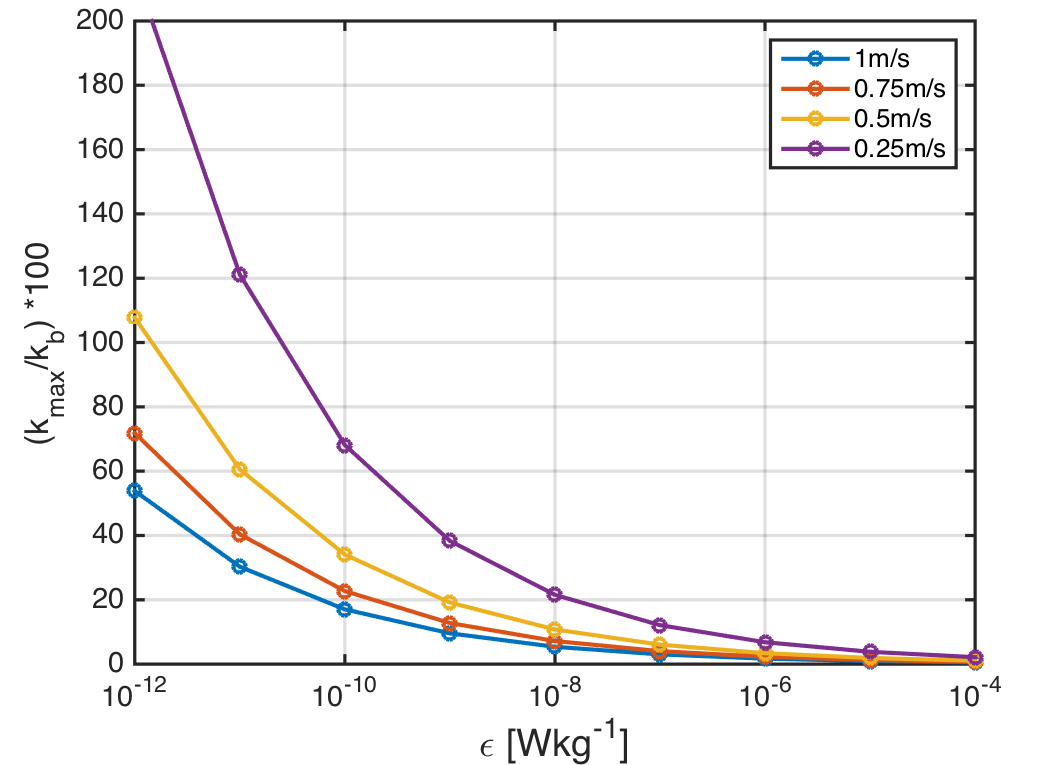
\includegraphics[width=38pc,angle=0]{kbratVsEps.png}\\
  \caption{Ratio of the maximum observed wavenumber $k_{max}=f_{max}/u$ to the Batchelor wavenumber $k_b$ for different values of $\epsilon$, assuming a $f_{max}=7Hz$. Each line is for a different flowspeed.}
  \label{kbratVseps}
\end{figure}

%\begin{figure}[t]
%  \noindent\includegraphics[width=38pc,angle=0]{p_loops2.png}\\
%  \caption{Example of pressure loops during different sea states. *Not sure if we need this.*}
%  \label{}
%\end{figure}

%PlotExampleTS.m
\begin{figure}[t]
  \noindent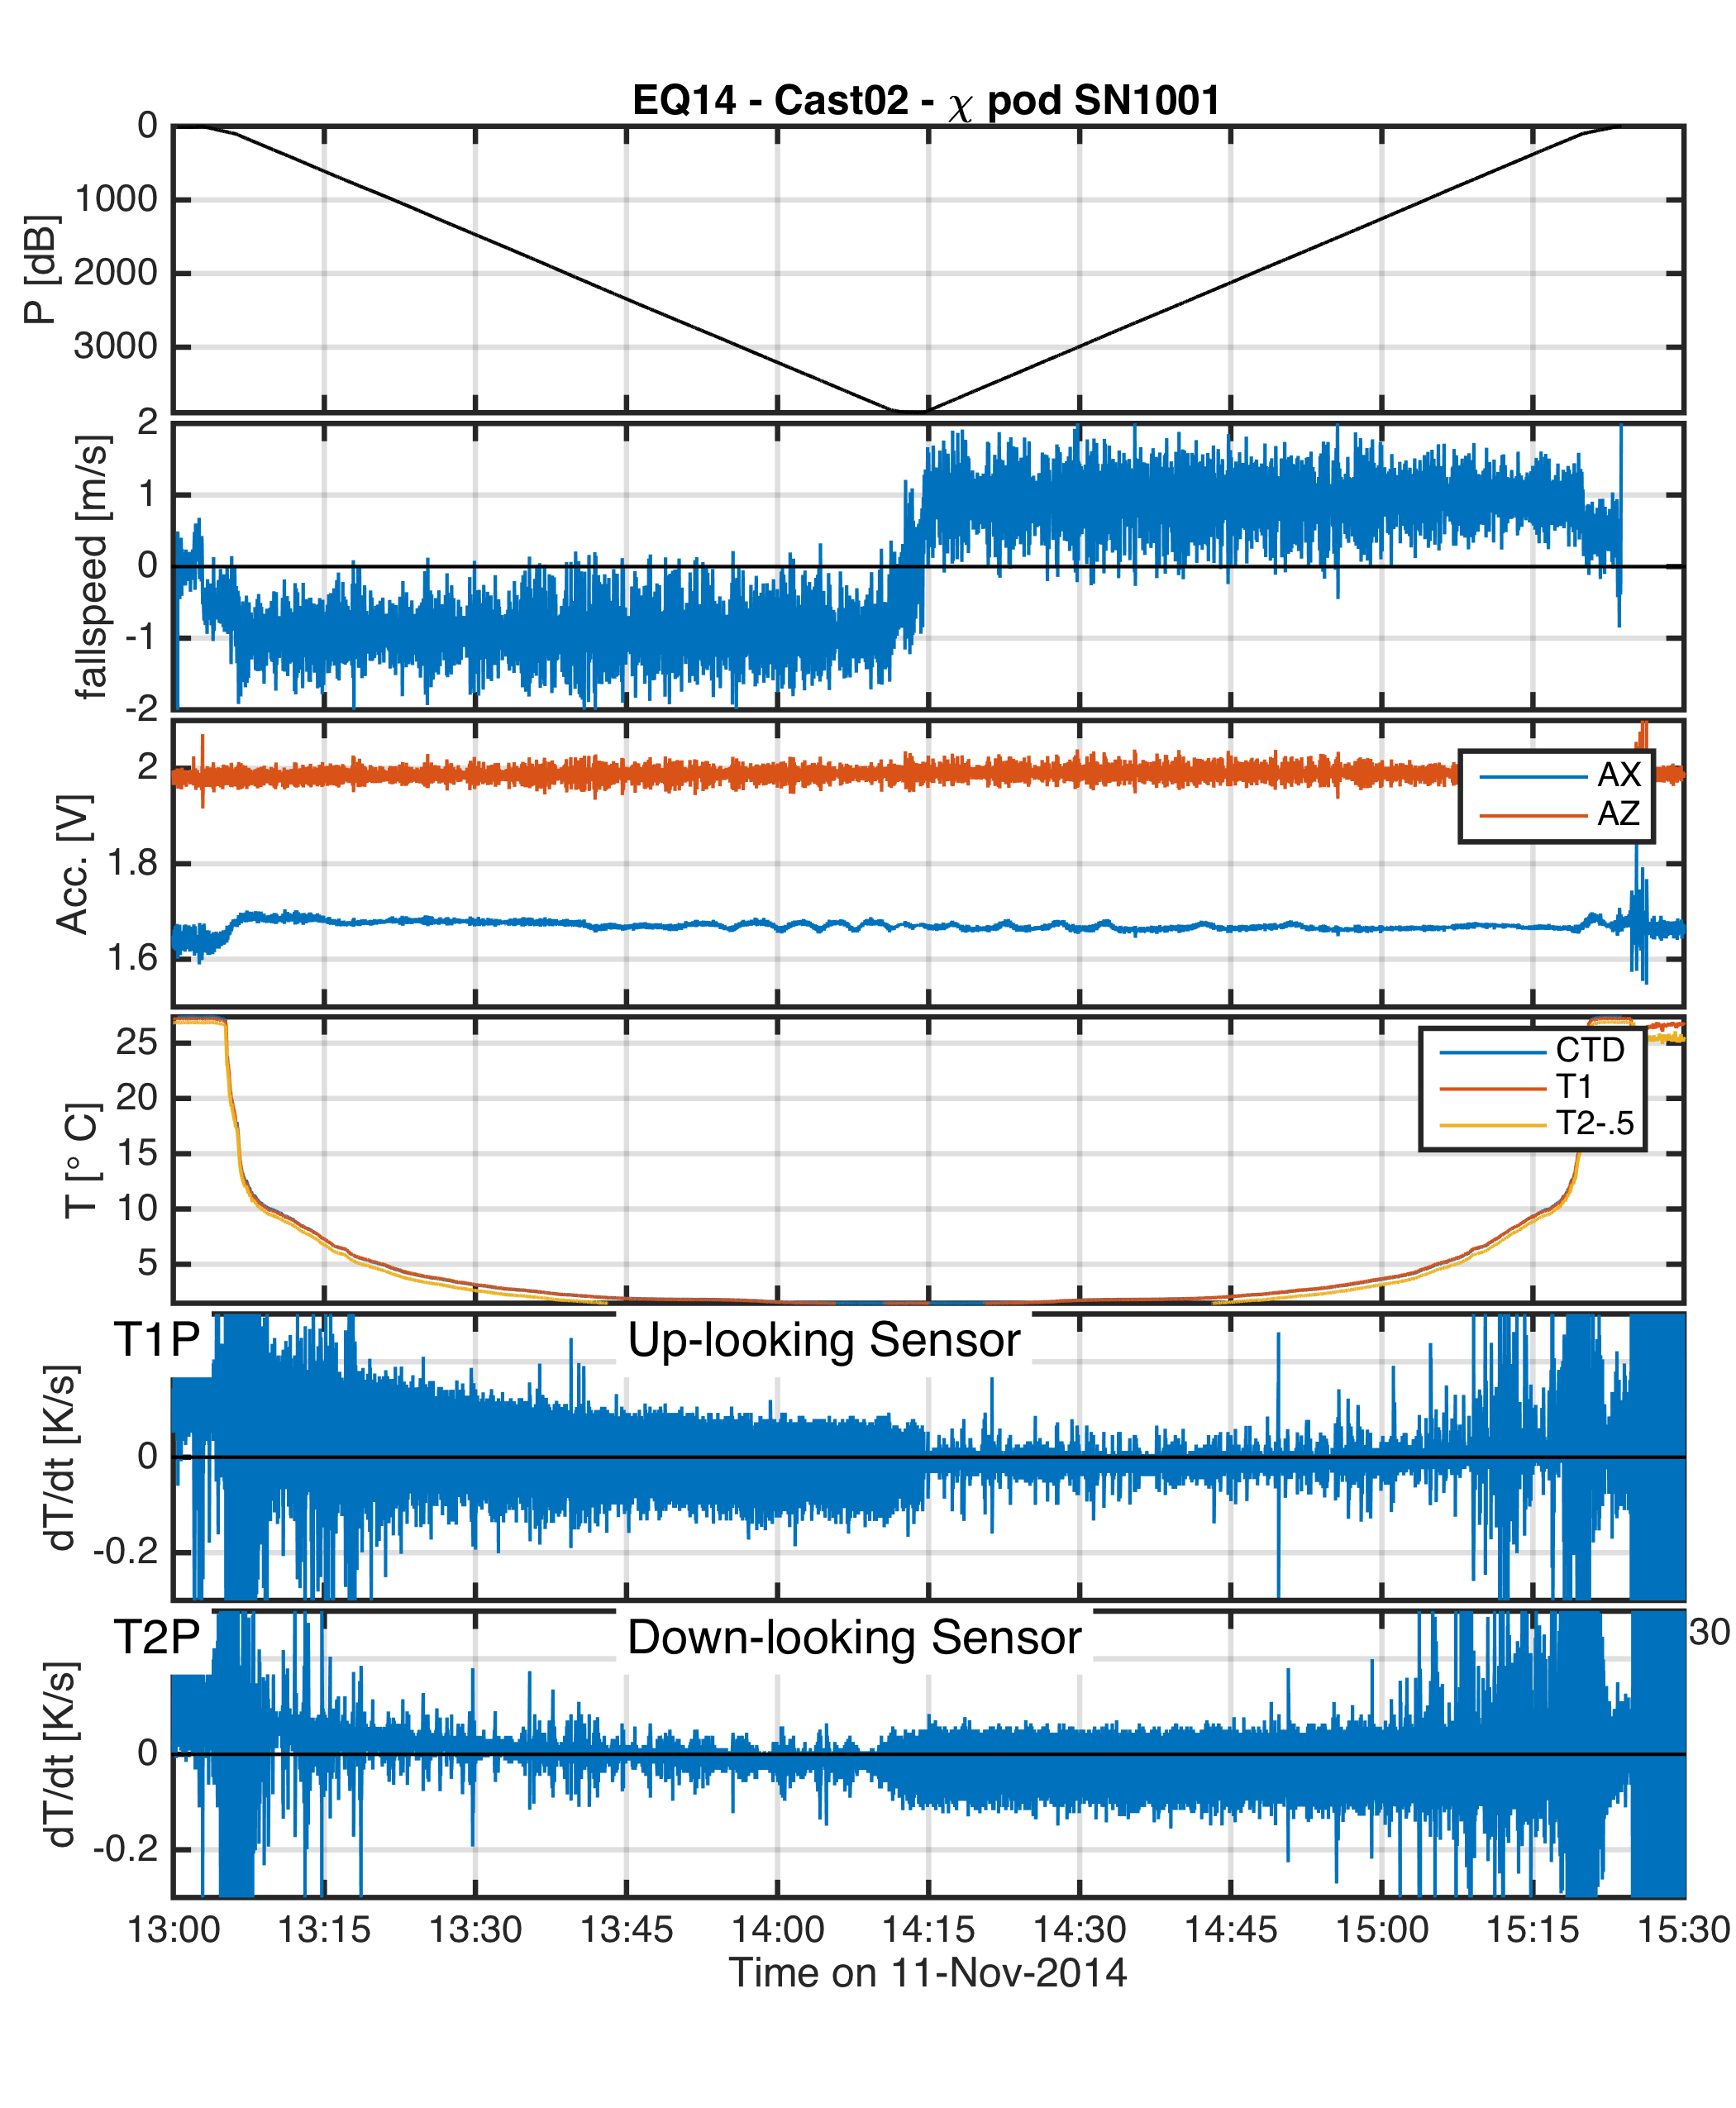
\includegraphics[width=38pc,angle=0]{SN1001_Cast02_Fig5_T_P_dTdz_fspd.png}\\
  \caption{Example timeseries from one CTD cast during EQ14. a) CTD pressure. b) Fallspeed of CTD ($dp/dt$) .c) Vertical and horizontal accelerations measured by $\chi$-pod. d) Temperature from CTD and (calibrated) $\chi$-pod sensors. T2 is offset slightly for visualization. e) Temperature derivative $dT/dt$ measured by the upward-looking $\chi$-pod sensor T1. f) Temperature derivative $dT/dt$ measured by the downward-looking $\chi$-pod sensor T2. **calibrate,add AX units. is it really -dT/dt? add 'up/down' looking labels for T' panels.}
  \label{f2}
\end{figure}



\begin{figure}[t]
  \noindent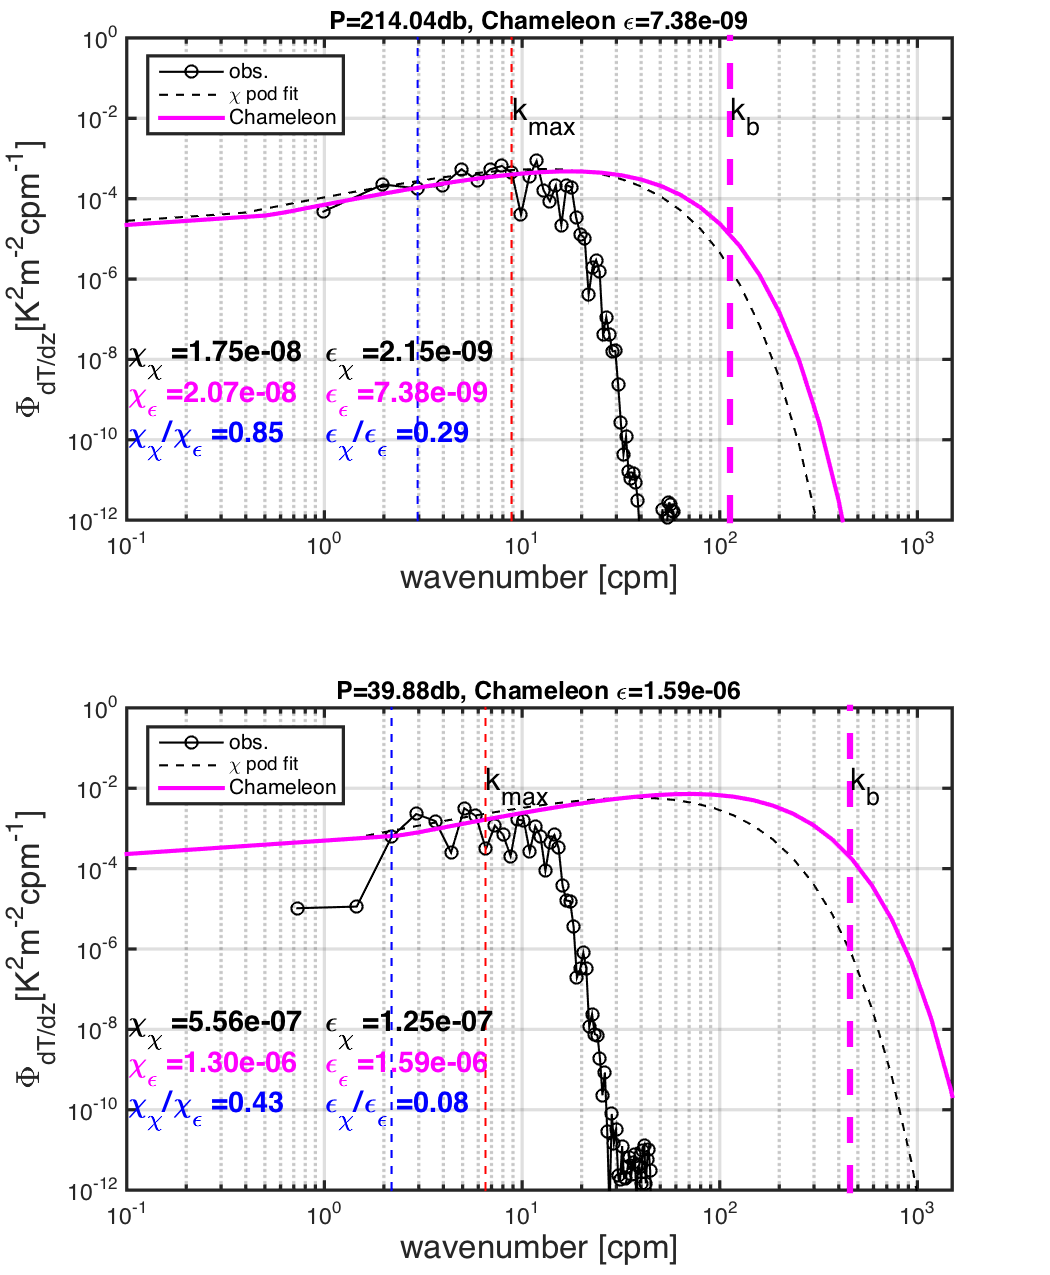
\includegraphics[width=38pc,angle=0]{ExSpec_HiLowEps.png}\\
  \caption{Example temperature gradient spectra from EQ14, for high (top) and low (bottom) $\epsilon$. Solid black line show the observed spectra. Dashed line shows the fitted theoretical Kraichnan spectra for the $\chi$pod estimates. Magenta line is Kraichnan spectra for Chameleon $\chi$ and $\epsilon$. Vertical dashed blue lines indicate the minimum and maximum wavenumber used in the $\chi$pod calculation. The Batchelor wavenumber $k_b$ is also indicated by the cyan line.}
  \label{specexamp}
\end{figure}


% Plot_chiProc_vs_actual_EQ14
\begin{figure}[t]
  \noindent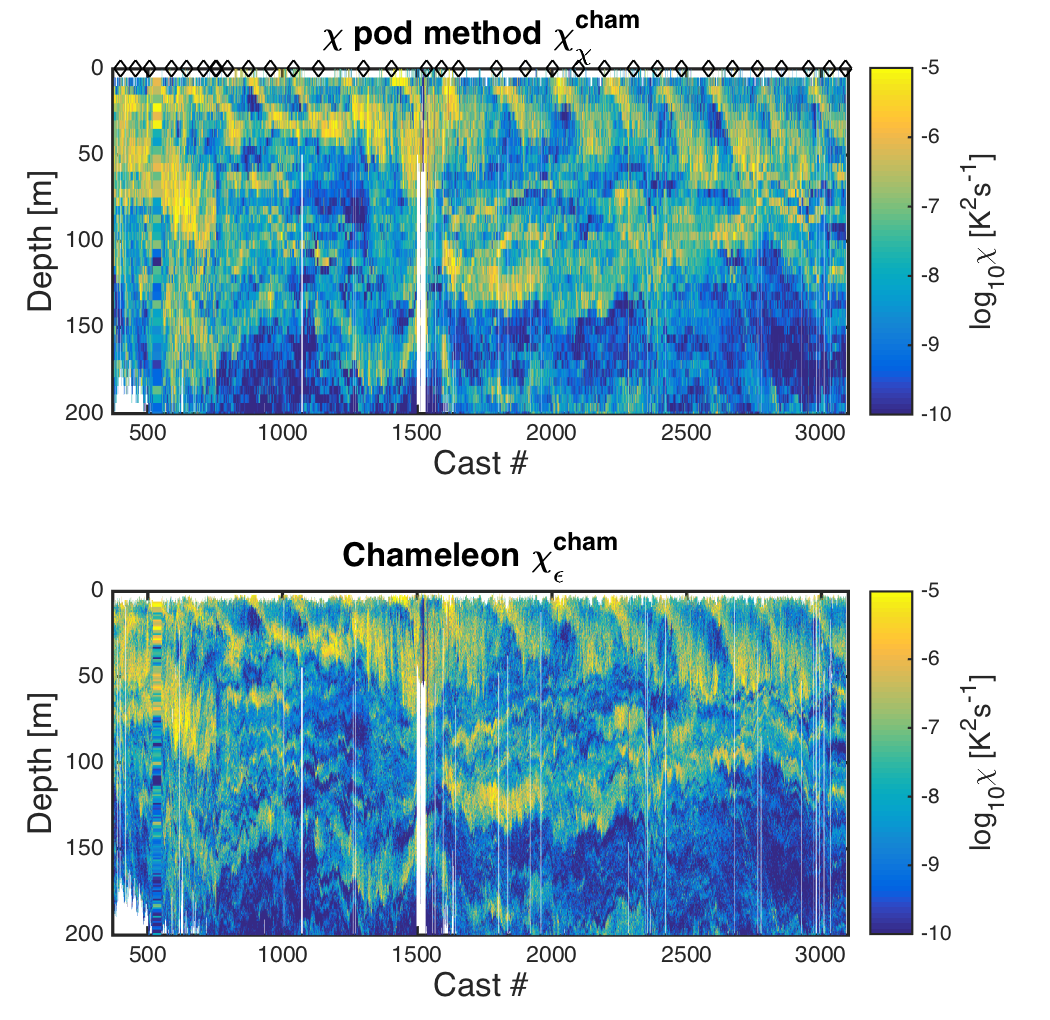
\includegraphics[width=38pc,angle=0]{EQ14_chiVsTrue_chi_zsm10m_fmax7Hz_respcorr0_fc_99hz_gamma20.png}\\
  \caption{Depth-time plots of $log_{10}\chi$ from both methods for EQ14 data. Top: $\chi$pod method. Black diamonds indicate casts used for comparison with CTD-$\chi$pod profiles. Bottom: Chameleon.}
  \label{eq14_eps_pcolor}
\end{figure}


\begin{figure}[t]
  \noindent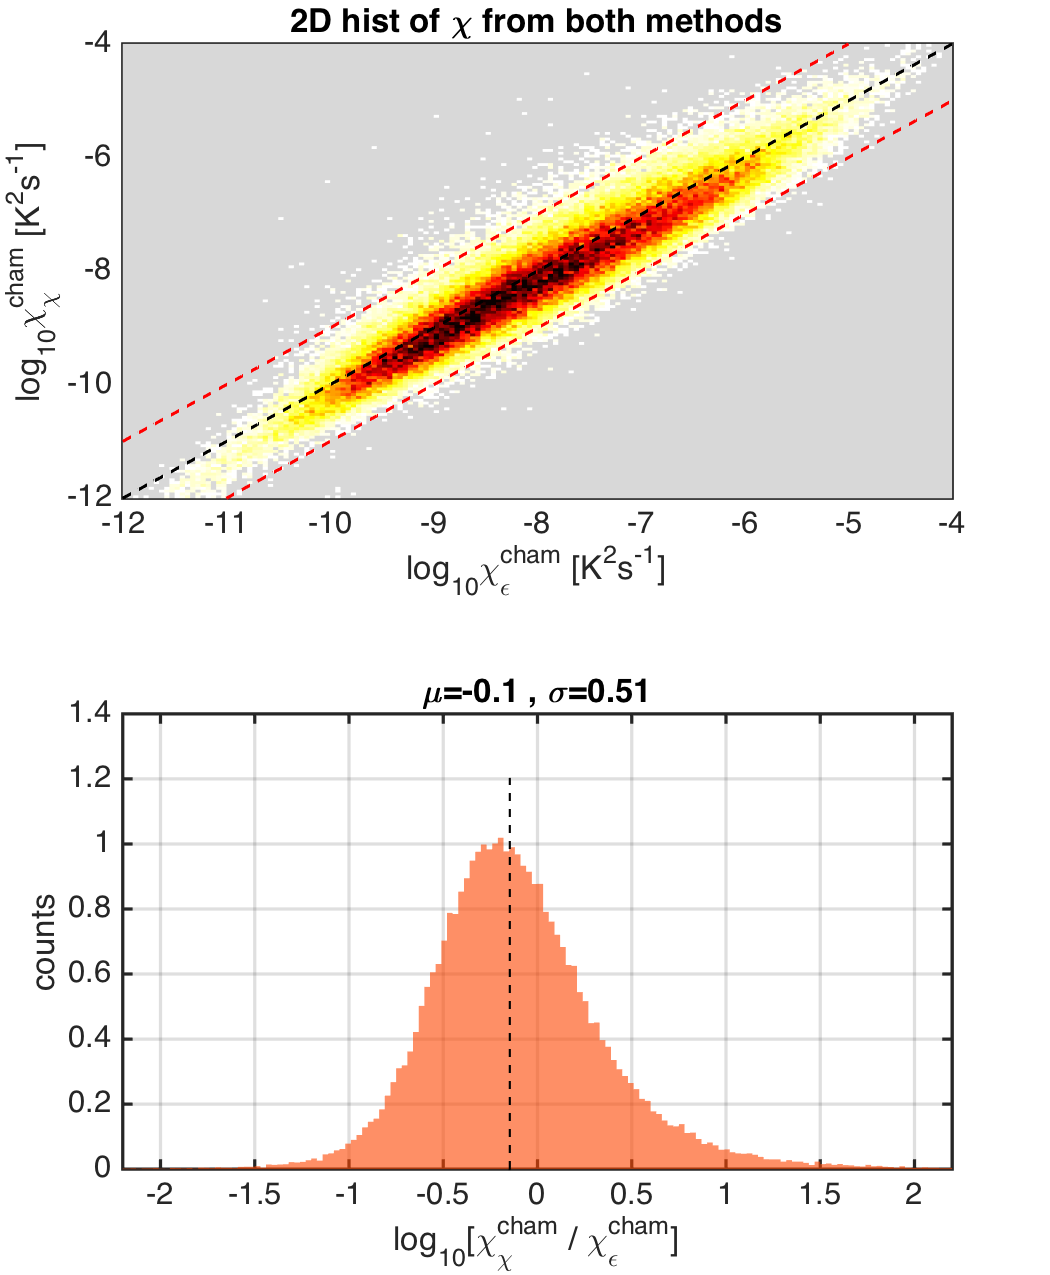
\includegraphics[width=38pc,angle=0]{EQ14_2dhist_chi_WITHhist_zsm10m_fmax7Hz_respcorr0_fc_99hz_gamma20.png}\\
  \caption{2D histogram of $log_{10}(\chi)$ from Chameleon (x-axis) and $\chi$pod method (y-axes). Values from each profile were averaged in the same 5m depth bins. }
  \label{eq14_chi_2dhist}
\end{figure}


% PlotHistKbRatio.m
\begin{figure}[t]
  \noindent\includegraphics[width=38pc,angle=0]{Hist_kbrat.png}\\
  \caption{Histogram of the (left) ratio of the maximum observed wavenumber $k_{max}$ to the Batchelor wavenumber $k_b$, and (right) fspd for all profiles in EQ14. }
  \label{histkbrat}
\end{figure}

%Scatter_CTDchiVsCham_Pairs.m
\begin{figure}[t]
  \noindent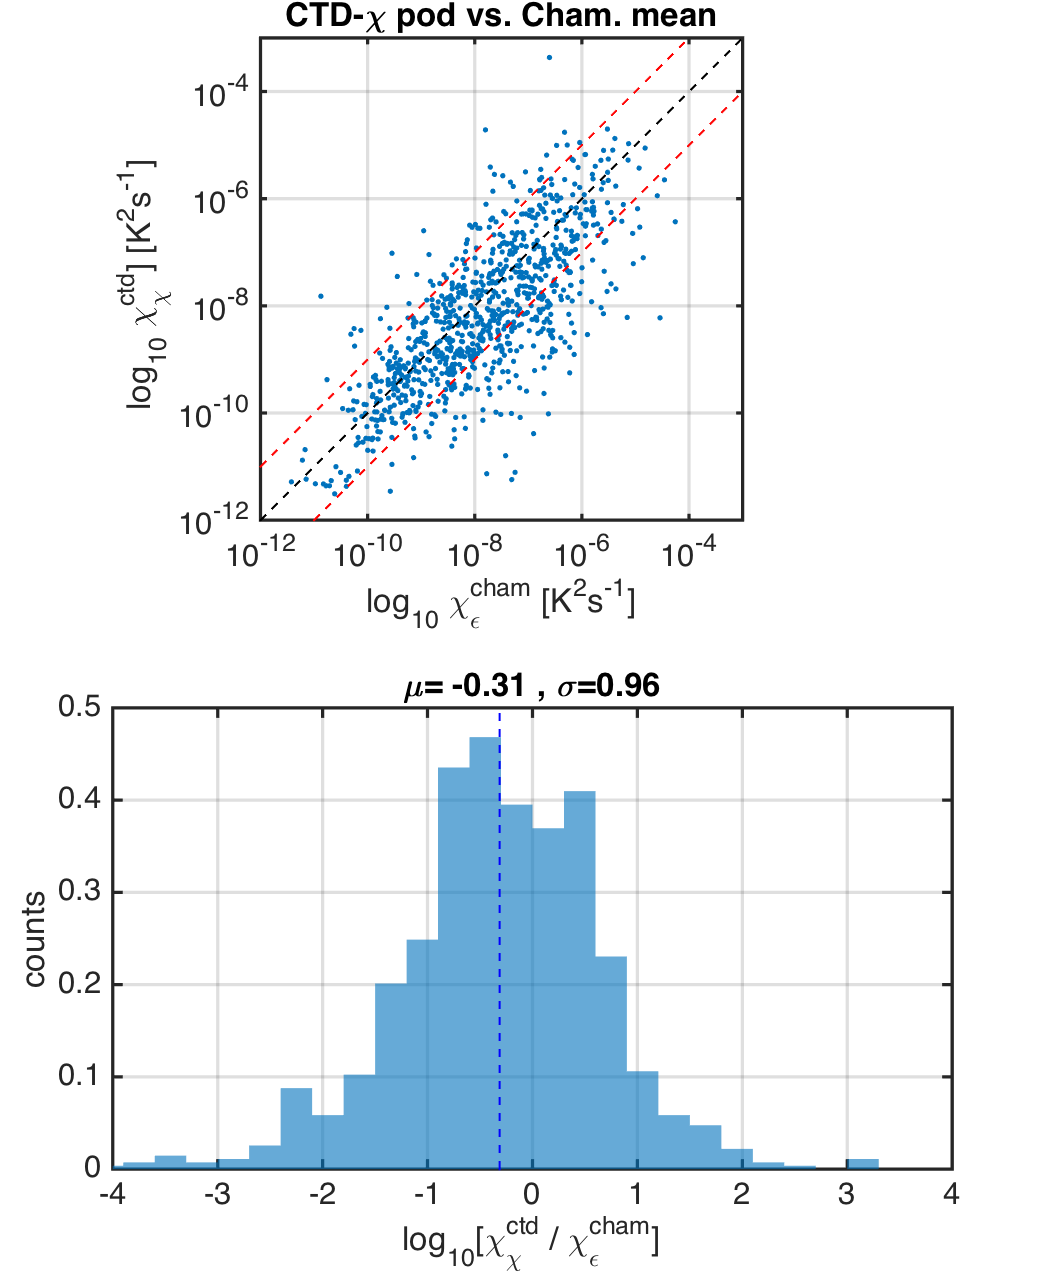
\includegraphics[width=38pc,angle=0]{EQ14_ctdChipod_vs_chamMean_chi_scatter_WITHhist.png}\\
  \caption{Scatter plot of $\chi$ from CTD-$\chi$pod profiles versus the mean of bracketing Chameleon profiles. Black dashed line shows 1:1, red are $\pm$ 10 X. **replace with histogram of ratios, or combine into one figure?**}
  \label{eq14_cdtChi_vs_cham}
\end{figure}

%Make_Combined_Cham_for_CTD_pairs.m
% PlotHistChiRatio_CTDchamPairs.m
\begin{figure}[t]
  \noindent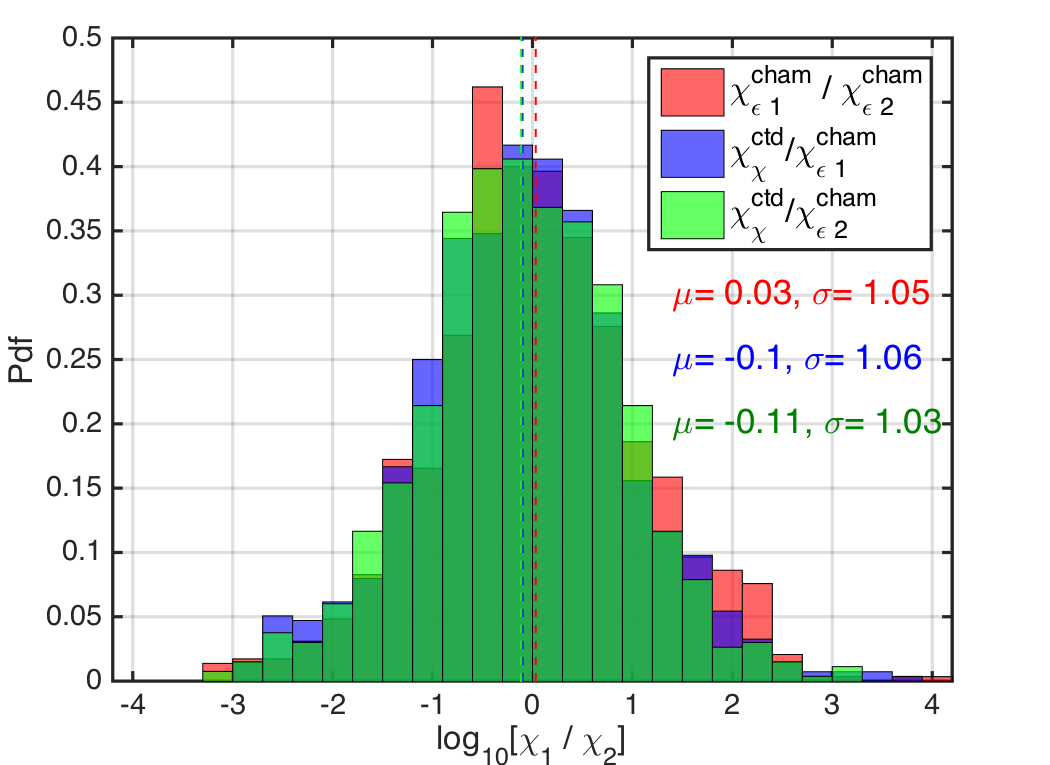
\includegraphics[width=38pc,angle=0]{EQ14_CtdChipod_hist_chi_ratios.png}\\
  \caption{Histogram of $log_{10}$ of the ratio of $\chi$ for nearby casts. The first set is for the before (cham1) and after (cham2) Chameleon profiles. the 2nd is CTD-$\chi$pod profiles versus the before(cham1) profiles. The last is CTD-$\chi$pod profiles versus the after(cham2) profiles. Dashed lines show the medians of each set.  Note that bias is small/zero, and the variability (spread) between CTD/cham is similar to the natural variability between cham profiles.}
  \label{eq14_cdtChi_vs_cham_hist}
\end{figure}

% Plot_Pairs_MeanProfile.m
\begin{figure}[t]
  \noindent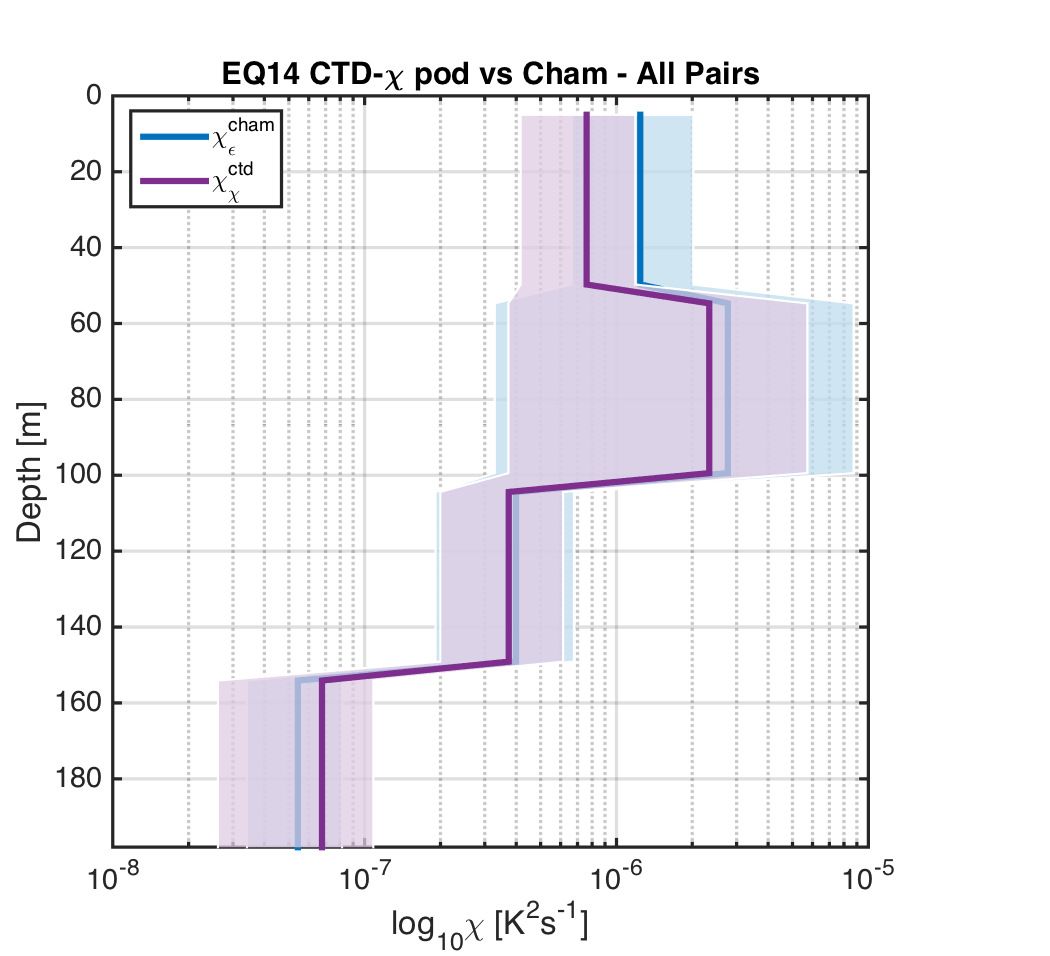
\includegraphics[width=38pc,angle=0]{EQ14_chi_cham_meanProf_all.png}\\
  \caption{Time mean of $\chi$ for all CTD-$\chi$pod - Chameleon cast pairs, with 95\% bootstrap confidence intervals.}
  \label{ctd_cham_chi_boot_all}
\end{figure}

% PlotP16chi.m
%\begin{figure}[t]
% \noindent\includegraphics[width=38pc,angle=0]{P16N_chi.png}\\
% \caption{Example chipod data from P16N. Top: dTdz. Bottom: $\chi$.}
% \label{p16ex}
%\end{figure}

\begin{figure}[t]
  \noindent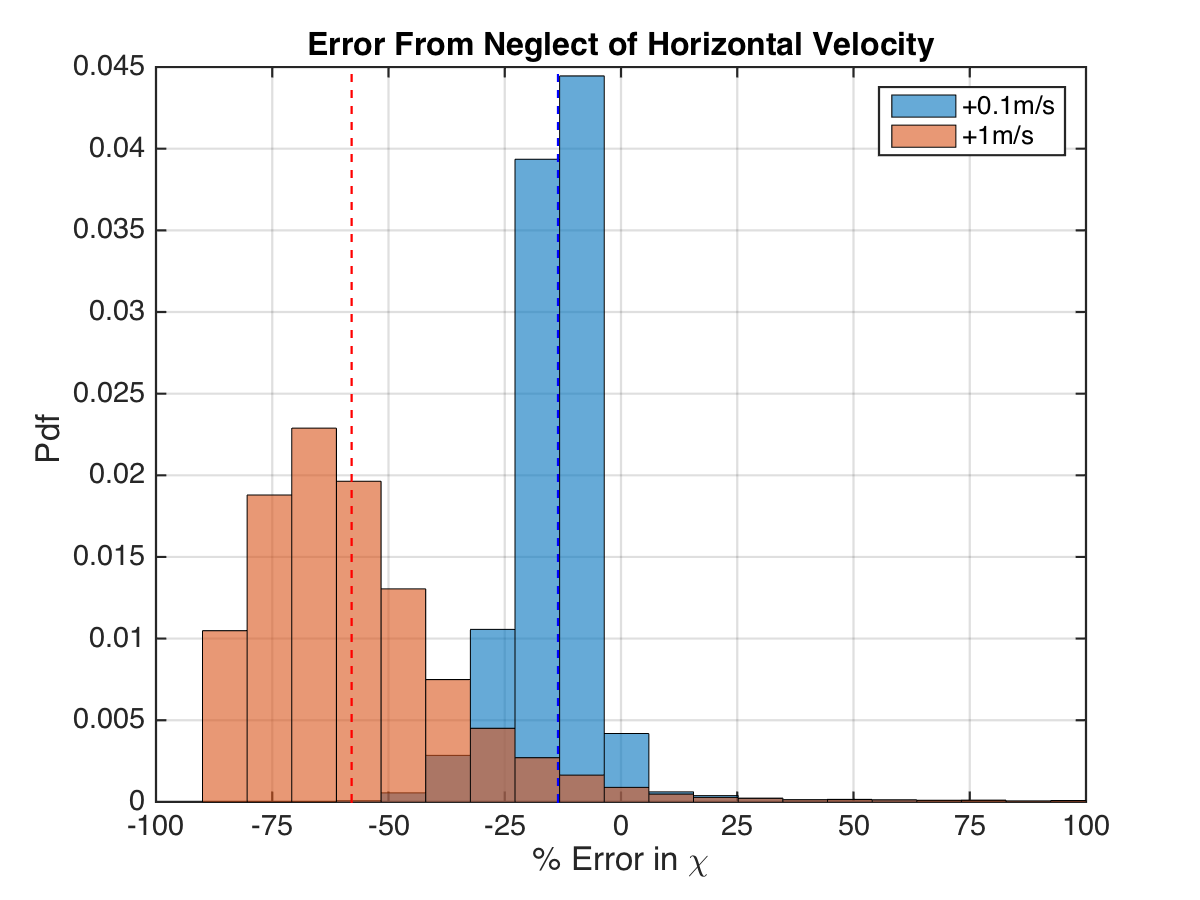
\includegraphics[width=38pc,angle=0]{Hist_perr_fspdvary.png}\\
  \caption{Histogram of \% error for $\chi$ computed with constant added to fallspeed, in order to examine sensitivity to fallspeed.}
  \label{FspdSensHist}
\end{figure}


\begin{figure}[t]
  \noindent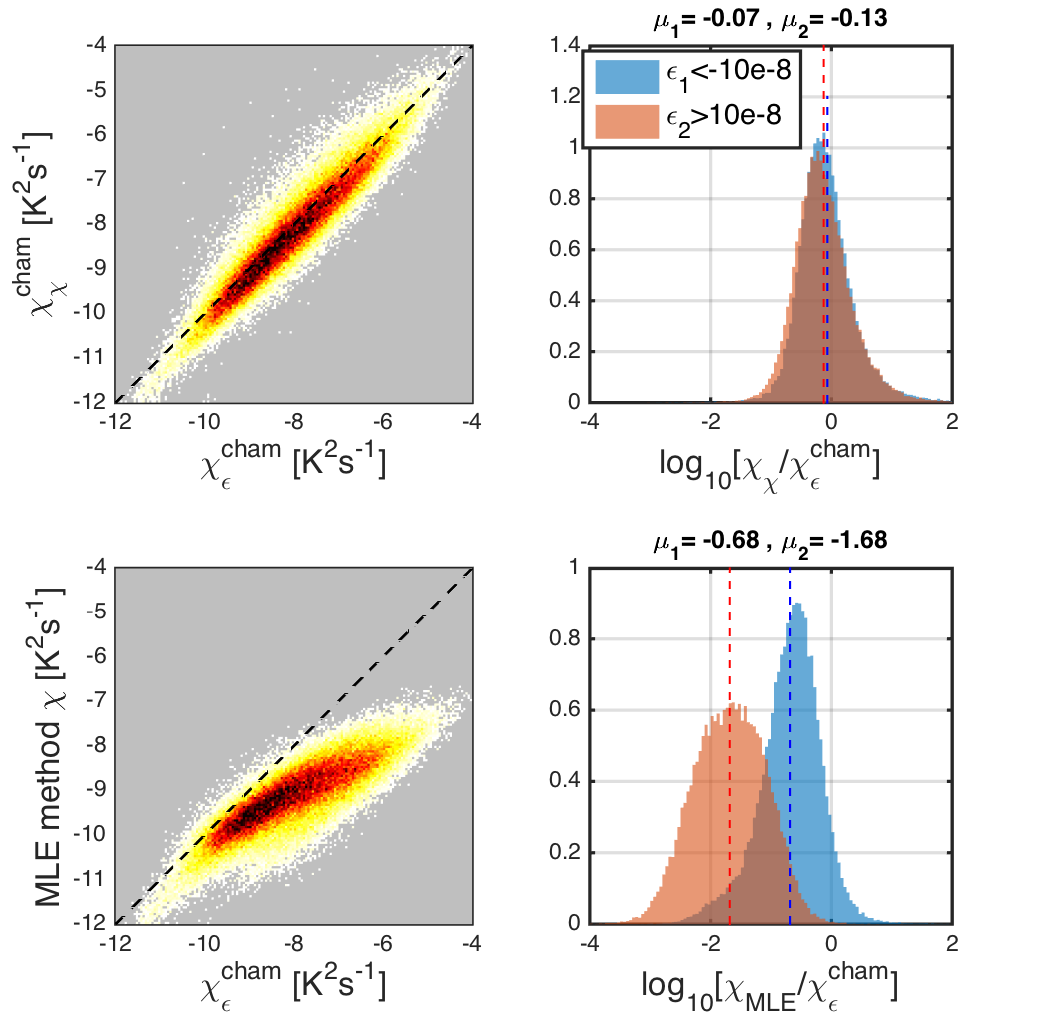
\includegraphics[width=38pc,angle=0]{MLEfitsEQ14_Whist.png}\\
  \caption{2D histograms of $\chi$ computed using the interative $\chi$-pod method (top) and the MLE fit (bottom) versus $\chi$ computed from Chameleon. Note that the MLE method underestimates $\chi$ at larger magnitudes.}
  \label{mlefits}
\end{figure}


\begin{figure}[t]
  \noindent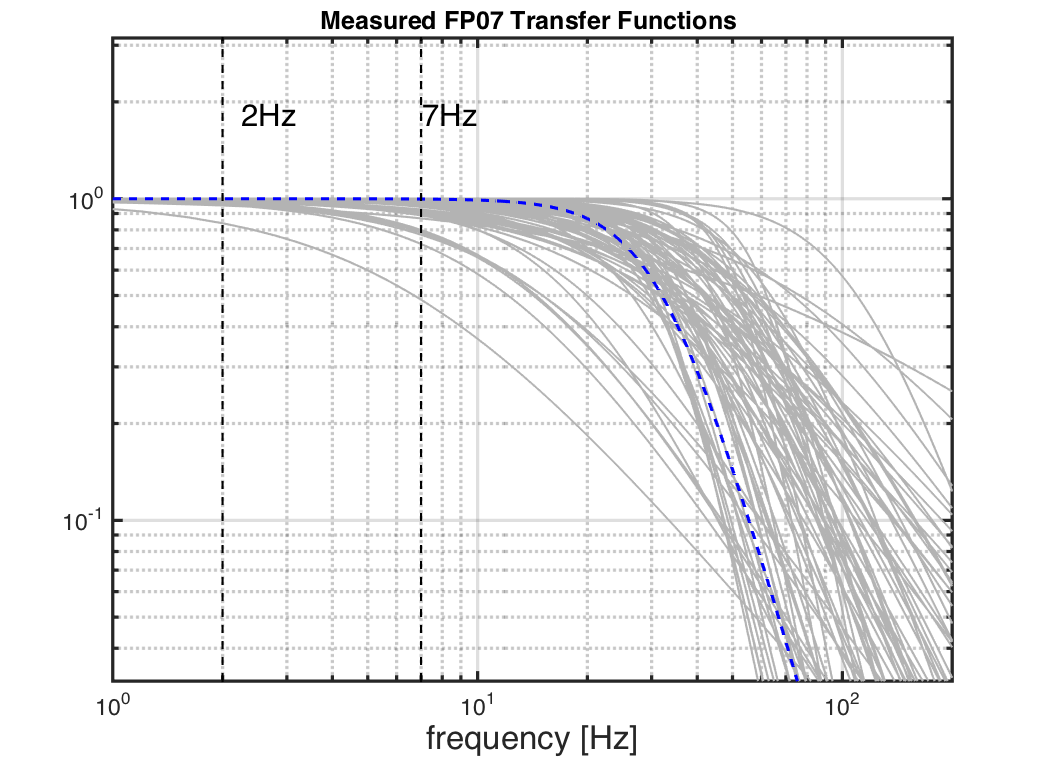
\includegraphics[width=38pc,angle=0]{yq08a_TransFunc.png}\\
  \caption{Measured FP07 thermistor transfer functions from historical database. Vertical dashed lines show the frequency range used in $\chi$pod method. Dashed blue line is a generic transfer function found to best match measured functions, and is used when response functions are no longer measured.}
  \label{xfr}
\end{figure}

%\begin{figure}[t]
%  \noindent\includegraphics[width=38pc,angle=0]{EQ14_boxplot_PctVar_xfr.png}\\
%  \caption{Boxplots of the \% variance of spectra captured using no transfer function over two different ranges of frequencies. Based on transfer functions in figure \ref{xfr}. }
%  \label{xfr2}
%\end{figure}




\end{document}